\documentclass[a4paper, 12pt]{article}

\usepackage[english,russian]{babel}
\usepackage[T2A]{fontenc}
\usepackage[utf8]{inputenc}
\usepackage{geometry}
\usepackage{enumitem}
\usepackage{setspace}
\usepackage{amssymb}
\usepackage{graphicx}
\usepackage{wrapfig}
\usepackage{float}
\usepackage{amsmath}
\usepackage{textcomp}
\usepackage{dsfont}

\geometry{top=5mm, left=1cm}
%\setlength{\parindent}{0}
\renewcommand{\arraystretch}{1.2}
\linespread{1}

\begin{document}
    \begin{center}
        \textbf{Сферическая геометрия тест №5}\\
        Площадь двуугольника, площадь треугольника.
    \end{center}

    \textbf{ФИО:}

    \begin{center}
        \textbf{№ 1}
    \end{center}

     Две сферические прямые пересекаются под углом $\frac{\pi}{2}$.
    Найдите чему равны площади каждого двуугольника, образованного этими прямыми, и посчитайте их сумму,
    если радиус сферы $R=52$ см.

     \textbf{Решение}\\

    \begin{center}
        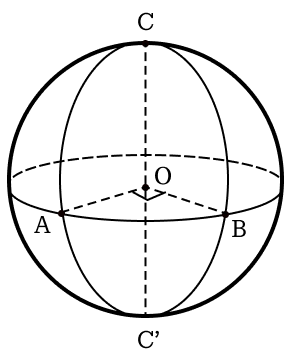
\includegraphics[width=0.2\textwidth]{images/img1}\\
    \end{center}

    1) Образуется четыре равных двуугольника, соответственно их площади равна:
    \[
        S = 2\frac{\pi}{2}R^2 = 2 \frac{\pi}{2} * 52^2 = 2704\pi \text{ см}^2
    \]

    2) Сумма всех двуугольников равна площади сферы, а именно:
    \[
        S_{sph} = 4\pi R^2   =10816 \text{ см}^2
    \]

    Ответ: $2704\pi \text{ см}^2$;  $10816 \text{ см}^2$

    \begin{center}
        \textbf{№ 2}
    \end{center}

    На сфере дан треугольник, два угла которого равны $\frac{\pi}{2}$, а третий равен $\frac{\pi}{3}$.
    Из вершины третьего угла на противолежащую сторону опустили медиану.
    Найдите площади получившихся треугольников, если радиус сферы равен $R$.

    \textbf{Решение}\\

    \begin{center}
        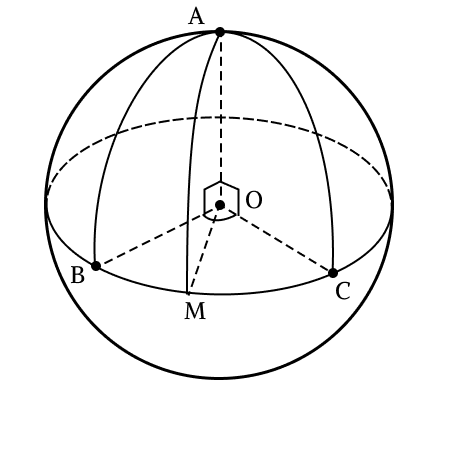
\includegraphics[width=0.2\textwidth]{images/img2}\\
    \end{center}

    1) $AO \bot (BOC)$ по признаку, тогда $(MOA)\bot(BOC)$ по признаку,

    2) \[
           \cup BM = \cup MC \rightarrow \angle BOM = \angle COM = \frac{\pi}{6}
    \]

    3)
    \[
        S = R^2(\angle BOM + \angle AOM + \angle AOB - \pi) = \frac{R^2\pi}{6}
    \]

    Ответ: $\frac{R^2\pi}{6}$

\end{document}
